\section{解の種類}
	この節では、指数関数と対数関数の交点を二種類に分類し、それらの存在する条件や性質について述べる。
	
\subsection{不動点解}
	$y = a^x$と$y = \loga x$はたがいに逆関数であるから、$a^x = x$を満たすような$x$、すなわち指数関数や対数関数の不動点は、$a^x = \loga x( = x)$となってこれらの交点の一つと分かる。
	このとき、$a = x^{\frac{1}{x}}$が成立する。
	このような$x$を不動点解と呼ぶこととする。
	また、$y = x,y = a^x$の増減から、端点を除いて$a > 1$では二つの不動点解が存在し、$0 < a < 1$では一つの不動点解が存在することが分かる。$a > 1$のときの、不動点解の大きい方を不動点大解、小さい方を不動点小解と呼ぶこととする。
	不動点解の存在する範囲を求めよう。
	\begin{theorem}
	\label{th:fixed_solutions}
		不動点解が存在するような$a$の範囲は$0 < a < e^\frac{1}{e}$である。
	\end{theorem}
	\begin{proof} \mbox{}\\
		$0 < a \leq 1$と$a > 1$のときで、場合分けをして考える。
		\begin{enumerate}
			\item $0 < a \leq 1$のとき
			
				$y = x$と$y = a^x$はどちらも単調に変化し、増減から$0 < x < 1$の範囲で一つ交点を持つので、不動点解を一つ持つ。
			\item $a > 1$のとき
			
				$y = a^x$のグラフを考えると、$a$を小さくしていくにつれてこれは直線$y = x$に近づき、いつか一点で接する。この接点において、
				\begin{align*}
					a^x &= x \quad (\text{二つのグラフの交点である}) \\
					a^x\ln{a} &= 1 \quad (\text{接線の傾き1})
				\end{align*}
				が成り立つから、これを解くと
				\begin{align*}
					a &= e^\frac{1}{e} \\
					x &= e 
				\end{align*}
				が得られる。
		\end{enumerate}
		これらより、\thref{th:fixed_solutions}が証明された。
	\end{proof}

\subsection{共役解}
	ところが、不動点以外でも指数関数と対数関数のグラフが交点を持つことがある。この解を共役解と定義し、小さい方から共役小解、共役大解とする。
	共役解には、一回底$a$で指数や対数を適用すると、もう片方の共役解が得られるという性質がある。
	共役解が存在することは以下のように証明できる。
	\begin{theorem}
	\label{th:conjugate_solutions}
		$0 < a < \frac{1}{e^e}$のとき、共役解が存在する
	\end{theorem}
	\begin{proof} \mbox{}\\
		このとき、\thref{th:fixed_solutions}より、不動点解$\xf$が区間$(0,1)$に存在する。
		$f(x) = a^x - \log_a x$とすると、
		\begin{align*}
			f(1) = a^x > 0 \\
			f(\xf) = 0
		\end{align*}
		だから、$f'(\xf) < 0$ならば、区間$(\xf,1)$に$f(x) = 0$を満たす$x$が存在するといえる。
		\begin{align*}
			f'(\xf) = a^{\xf}\ln a - \frac{1}{\xf\ln a} &< 0 \\
									 a^{\xf}\xf\ln^2 a  &> 1 \quad (\ln a < 0\text{より}) \\
											  \ln^2 \xf &> 1 \quad (0 < a^{\xf} = \xf < 1\text{から}) \\
												0 < \xf &< \frac{1}{e} \\
												  0 < a &< \frac{1}{e^e}
		\end{align*}
		したがって、\thref{th:conjugate_solutions}が証明された。
	\end{proof}
	
	実際にグラフを書くと図\ref{fig:three_roots_ex}や図\ref{fig:two_roots_ex}のように、共役解や不動点解が存在しているのが分かる。
	\begin{figure}[hbtp]
	\begin{minipage}{0.5\hsize}
		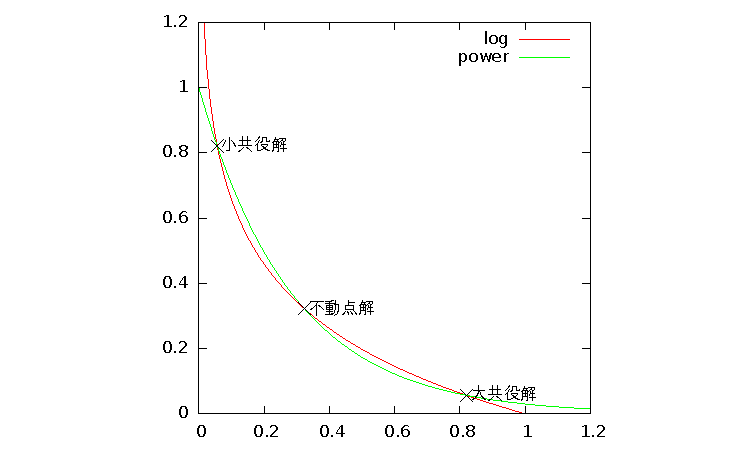
\includegraphics[width=80mm]{../plot/graph/three_roots_ex.pdf}
		\caption{$a \sim 0.03$}
		\label{fig:three_roots_ex}
	\end{minipage}
	\begin{minipage}{0.5\hsize}
		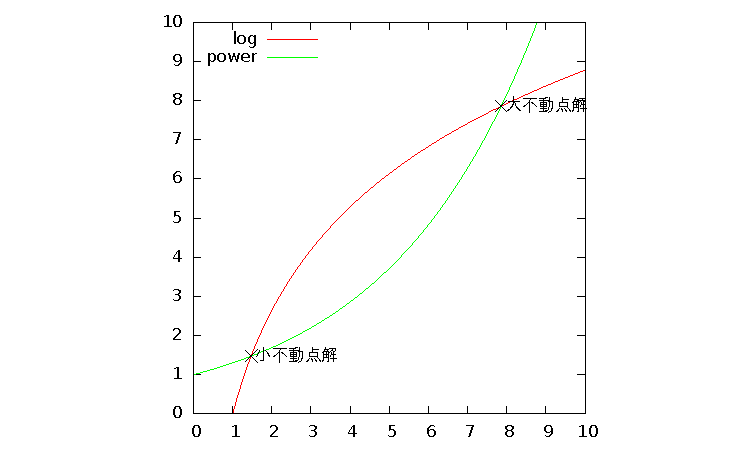
\includegraphics[width=80mm]{../plot/graph/two_roots_ex.pdf}
		\caption{$a \sim 1.3$}
		\label{fig:two_roots_ex}
	\end{minipage}
	\end{figure}
	
	
